\chapter{Component tree}\label{chapter:cptree} \label{chpt:cptree}
Componet tree is one of the main topic in my thesis for cell tracking. In my cell tracking algorithm, each image is converted into a component tree. Then the component trees are used for tree assignment based cosegmentation. Najman and Couprie \cite{Najman:04,najman2006building} proposed a fast way, which is based on Tarjan's union-find procedure, to build a component tree. However, the constructed component tree is usually very large, which is too large for later tree assignment step. It is observed that most nodes in the component tree are redundent which make the tree really big. In this thesis, I proposed a pruning method which decrease the final tree significantly (0.1\% of the original size).\\
Before component tree assignment, we need to compute the weights between every pair of nodes in two component trees. This step is extremely time consuming, which is once a bottle-neck of our cell tracking algorithm. However, we proposed a fast dynamic algorithm which enables a quasi-linear running time from $O(|T1|\cdot|T2|\cdot N)$ to $O(N)$.
\section{Component tree construction} \label{sec:cptree-def}
\subsection{Component tree definition}
A component tree $T$ can be described as $T=(V, E)$, where $V$ is the set of nodes (or component nodes) in tree $T$, and $E$ is the inclusion relationship between component nodes. Each component node is mapped to a connected area (or connected component or just component) under some threshold. The relationship between any two component nodes is either inclusion or non-overlaping. However, we only consider the relationship between two nodes $u$ and $v$. That is if area of $u$ includes area of $v$, there will be no other node whose area includes area of $v$ or is included by area of $u$. Fig.\ref{fig:cptree-example} shows the component tree of an very simple image, by considering five different threshold values.

In pratice, a component tree usually considers all threshold values with all possible connected components, which is called a \emph{full component tree}.

\begin{figure}[htbp]
\centering
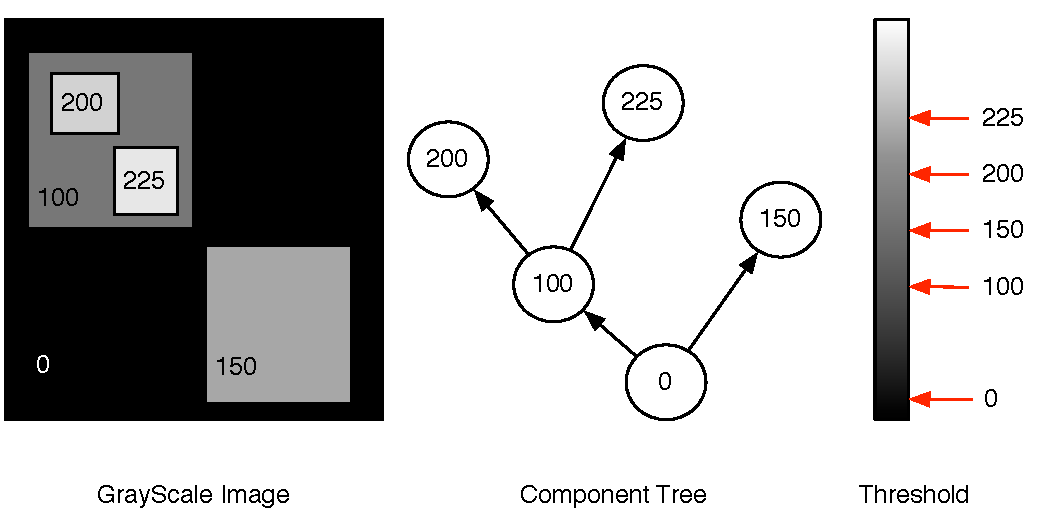
\includegraphics[width=1.0\textwidth]{images/cptree_example}
\caption[An example of component tree with four levels and five components]{The component tree with five different values. A. the original image; B. The corresponding component tree; C. the key threshold values}
\label{fig:cptree-example}
\end{figure}
\subsection{The $\alpha$ and $\beta$ area} \label{sec:alpha-beta-area}
Each node in the component tree is mapped to a connected area, which is denoted as its $\beta$ area. As the $\beta$ area includes the $\beta$ areas of all its child nodes, we can define the $\alpha$ area of a node which is its $\beta$ area exclusive of all its child nodes. Thus, for each node $v$, we have
$$
\beta(v) = \alpha(v)\cup\bigcup_{v_i \in C(v)} \beta(v_i)   
$$
$$
\alpha(v) = \beta(v) - \sum_{v_i\in C(v)}\beta(v_i)
$$
where $C(v)$ is all child nodes of $v$, $v_i$ is the $i_{th}$ child node of $v$. 

We can find the lowest intensity in the connected component which is called the \emph{level of the connected component}. Thereby, the $\alpha$ area of a component can also be defined as the set of pixels with intensity equal to the level of the component.
$$
\alpha(v) = \{p \in \beta(v)| I(p) = level(v)\}
$$
Fig.\ref{fig:cptree-alpha}A illustrates the relationship between $\alpha$ nodes and $\beta$ nodes. It is easy to prove that the $\alpha$ area of all possible component nodes is a partition of the whole image. 
$$
\bigcup \alpha(v) = I
$$

\begin{figure}[htbp]
\centering
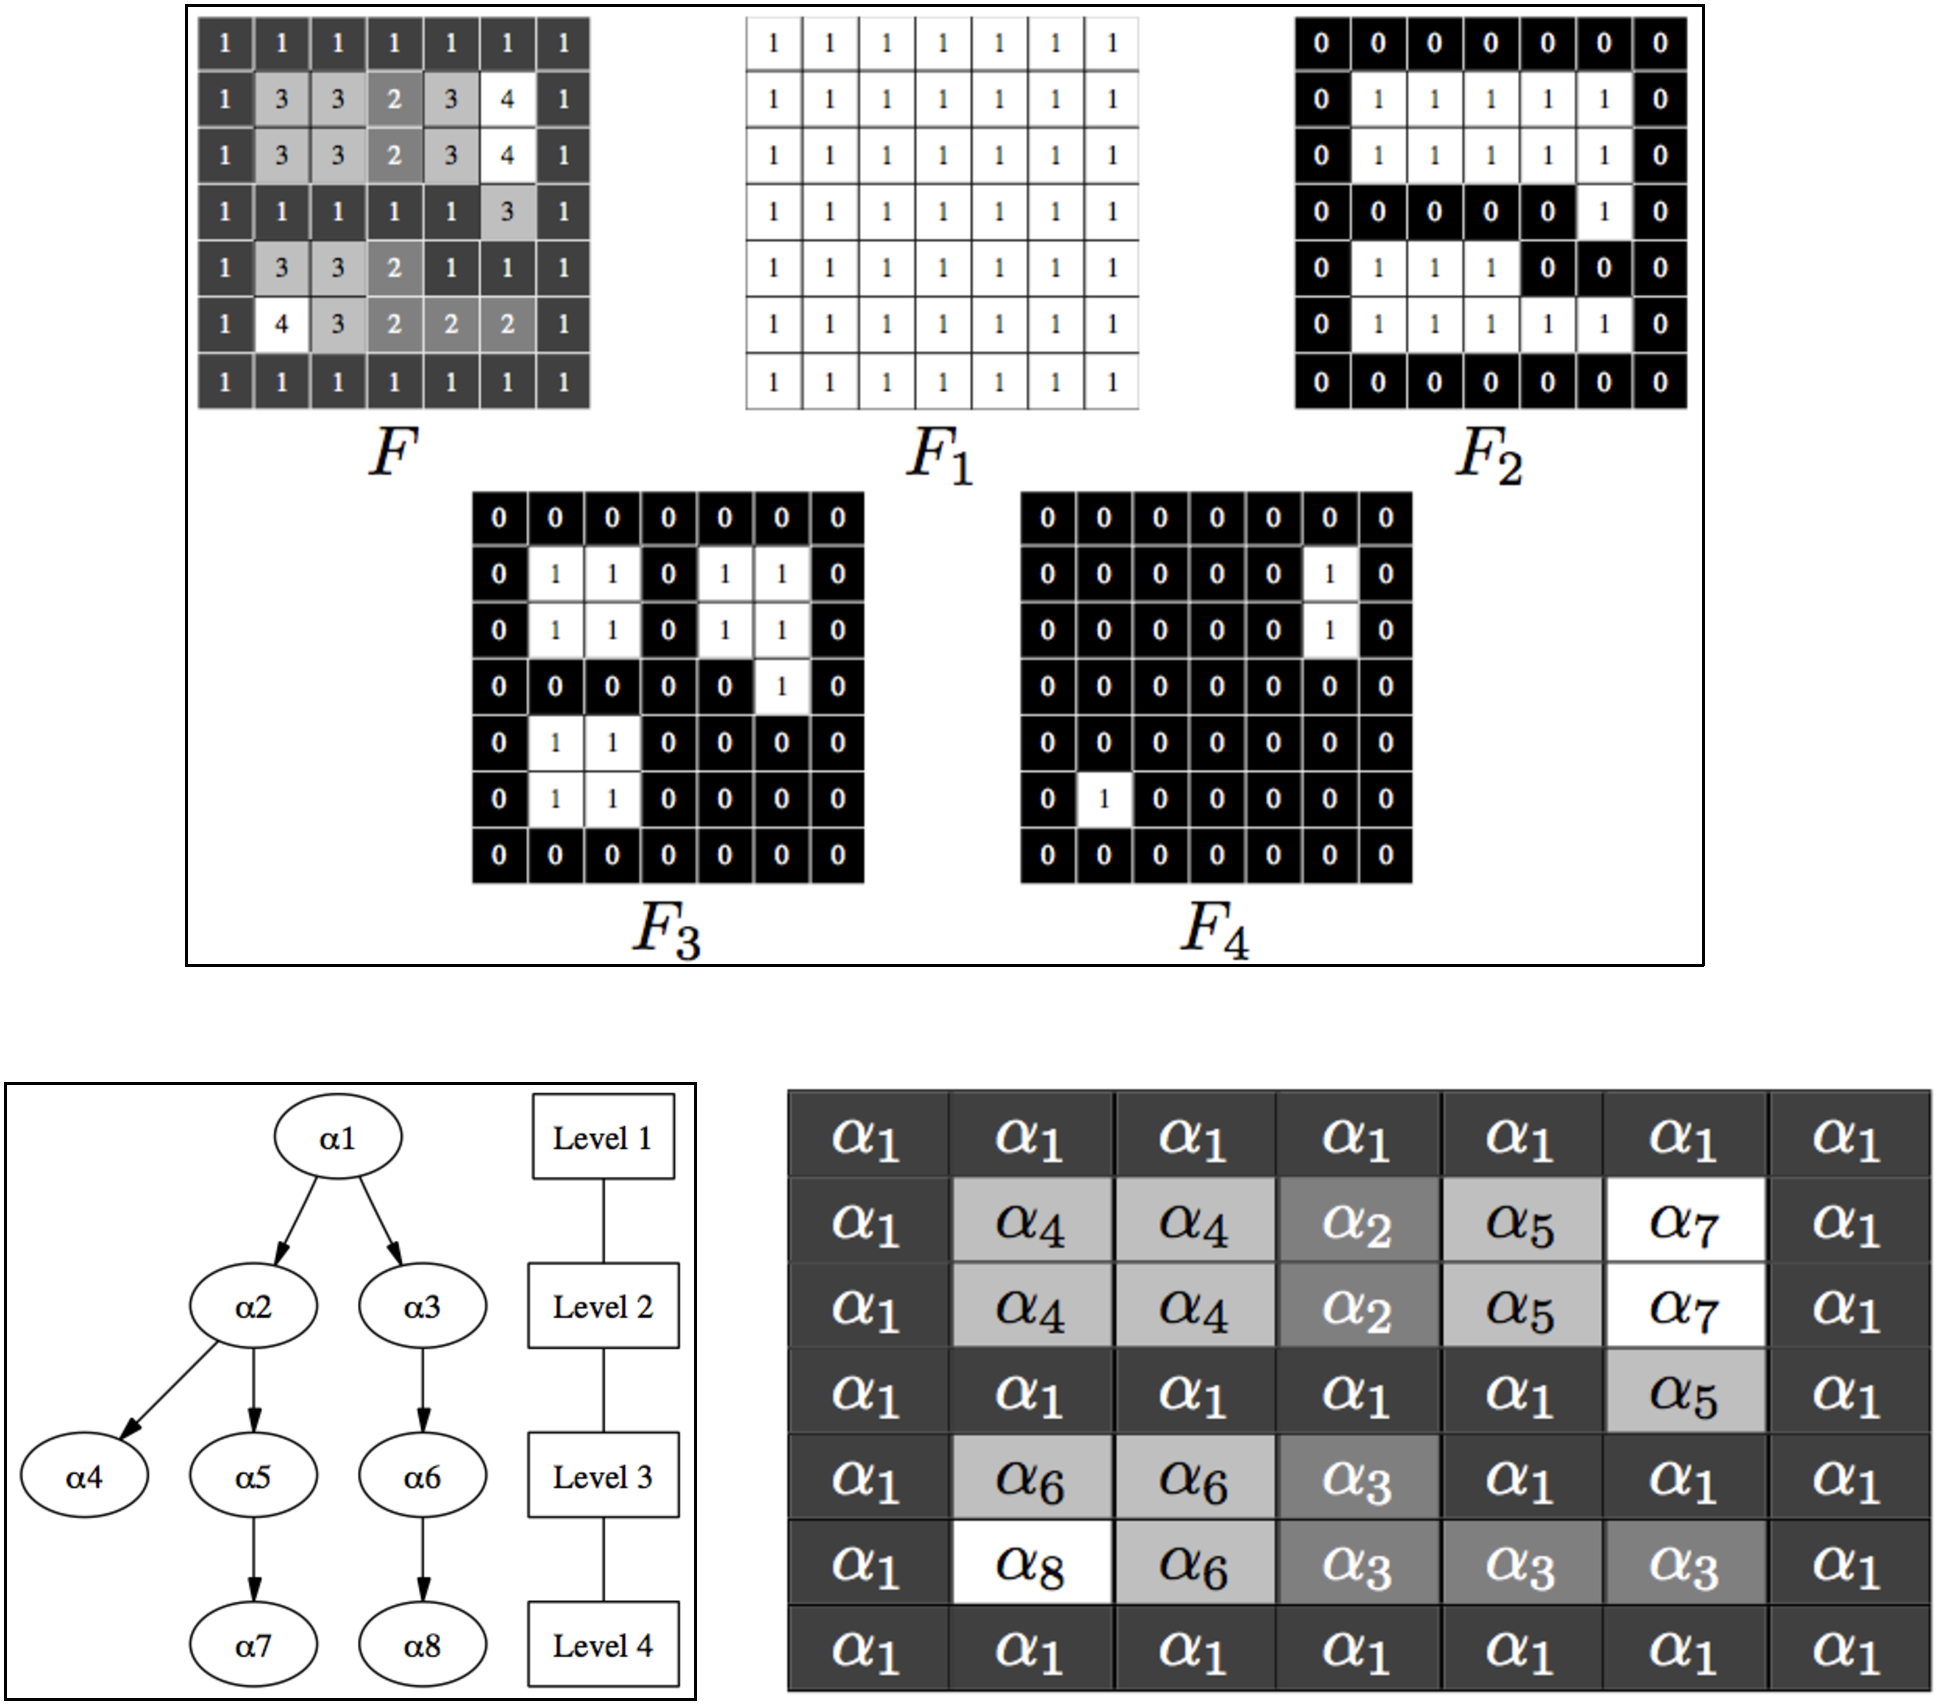
\includegraphics[width=1.0\textwidth]{images/cptree_alpha}
\caption[The $\alpha$ area and $\beta$ area of component tree node]{The $\alpha$ area and $\beta$ area of component tree node. A. The relationship between $\alpha$ nodes and $\beta$ nodes; B. The mapping between pixels to component nodes.}
\label{fig:cptree-alpha}
\end{figure}

As there is no overlap between the $\alpha$ area of any pair of nodes, each image pixel can be mapped to a component node uniquely. Fig.\ref{fig:cptree-alpha}B illustrates the mapping of $\alpha$ node.

\subsection{Quasi-linear algorithm}
The process of constructing component tree is a process of partition the image into many non-overlapping areas ($\alpha$ areas) with relationship. According to this idea, Najman and Couprie\cite{najman2006building} proposed a quasi-linear time to construct a component tree. They utilize the disjoint-set data structure  to represent the discreted $\alpha$ areas.

The algorithm needs only one searching of all image pixels in the order of there intensity from highest to lowest. Initially every image pixel is mapped to a disjoint set (element) with parent to itself. And each disjoint set is mapped to a component node with only one pixel, both for its $\alpha$ area and $\beta$ area and no child node. That's to see, each image pixel is mapped to a component node through its mapped disjoint set.

When one image pixel with intensity $T$ is processed, we will first find its corresponding disjoint set and component node, see \emph{current component node}; then we check its neighboring pixels. If the neighboring pixel is of intensity larger than $T$, add the component node of the neighboring pixel to the child of current component node. If the neighboring pixel is of equal intensity to $T$, we merge both the disjoint set and child component nodes of both pixles. See alg.\ref{alg:cptree-quasi} for algorithm details.

\textbf{Implementation: } During the implementation, I find it hard to get the elements of a disjoint set (or the $\alpha$ area) with only parent and rank information. However, by adding a next node information, wo solve the problem. The next node information link all the elements of a set in a loop, which enabls geting the whole set from any element.

\textbf{Running time: } Let $N$ denotes the number of image pixels. The first step is sorting the image pixels. It can be done in $O(N)$ if the weights are small integers \cite{cormen2001introduction}. In the looping, both adding childs and merging childs and merging disjoint set can be done in constant time. So the total running time is quasi-linear of $O(N)$.

\begin{algorithm}[H]
\SetAlgoLined
\KwData{An image $I(x,y)$}
\KwResult{A component tree of the image}
Sort the image pixels from highest to lowest\;
Create a disjoint set for each image pixel, and build the mapping $pixel2djs$ from image pixel to disjoint set\;
Create a component node for each disjoint set, and build the mapping $djs2node$ from the disjoint set to the component node\;
\ForEach{pixel in sorting order}{
	Find the intensity $T$ of current pixel\;
	Find the disjoint set $cur\_djs$ of current pixel from $pixel2djs$ mapping\;
	Find the component node $cur\_node$ of $cur\_djs$ from $djs2node$ mapping\;
	\ForEach{pixel neighbors to current pixel}{
		Find the intensity $T'$ for the neighboring pixel\;
		Find the disjoint set $nei\_djs$ of neighboring pixel from $pixel2djs$ mapping\;
		Find the component node $nei\_node$ of $nei\_djs$ from $djs2node$ mapping\;
		\If{$T' > T$}{
			Add $nei\_node$ as a child of $cur\_node$\;
		}
		\ElseIf{$T' == T$}{
			Merge $nei\_djs$ to $cur\_djs$ by union-find algorithm\;
			Delete the mapping of $nei\_djs$ in $djs2node$ mapping\;
			Add all the childs of $nei\_node$ to the childs of $cur\_node$\;
			Delete $nei\_node$\;
		}
	}
\caption{Build component tree with quasi-linear time}
\label{alg:cptree-quasi}
}

\end{algorithm}

\section{Component tree pruning}
Each image is uniquely mapped to a component tree, and vice versa. Usually the constructed component tree is extremly large (133187 nodes for a microglia image of size 156x250x34). But the tree assignment step only tolerant a tree of size about 200. It is absolutly necessary to prune the component tree before moving into next step.\\
\subsection{Redundancy rate}
The redundancy rate of a component tree is defined as the ratio between the size of component tree and that of its corresponding image. For an image of size $N$. The maximum redundancy rate is 100\% when each pixel maps to a component node. The minimum redundancy rate is $1/N$ when there is only one node in the tree with the pixels of the whole image. For the microglia above, 133187 nodes for an image of size 156x250x34, the redundancy rate is 10.04\%.\\
The redundancy rate reflects the structure complexity of an image. High redundancy indicates an nosiy image with many small components, whereas low rendundancy indicate a clear image with few big components. However, for a component tree with high redundancy rate, a proper pruning process could lower the redundancy rate and make the main structure, the objects that we are interested, clearlly represent in the pruned component tree.
\subsection{The redundant nodes}
Fortunately, we find lots of redundant nodes from the statistic of a full component tree. There are plenty of nodes with very few pixels and huge number of single nodes, which is the only child of its parent. Look at fig\ref{fig:cptree-random}, it is the full component tree of a random image of size only 10x10, but 79 nodes. The small nodes leads to lots of leaf nodes in the tree. The single nodes contribute most nodes for the tree and make the tree extremly long with high depth. \\
The small nodes usually means a noise component, which should be deleted without hesitation. The single node is created in the instance that when the threshold increase, a big component shrinks to a smaller compoent (the created single node) without breaking into pieces. A path with long single nodes from ancestral node to child node represents the size decreasing tendency of a big ancestral node. The single node without too much change from its parent is not very important and should be deleted.\\
Besides the two main kinds of redundant, there is a third kind of redundant nodes, that is the components with huger size which is more than the object size we are interested. 
\begin{figure}[htbp]
\centering
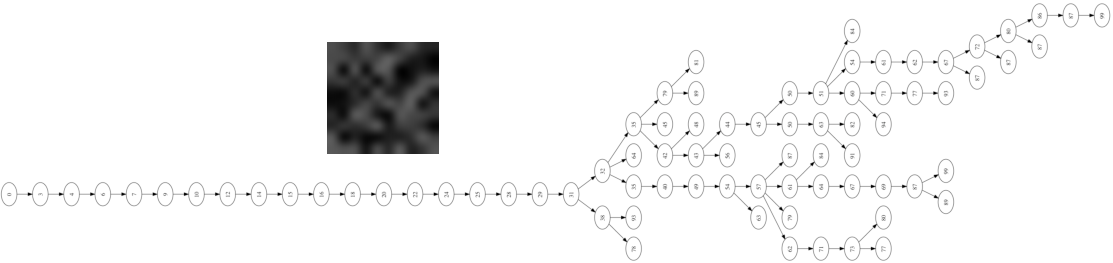
\includegraphics[width=1.0\textwidth]{images/cptree_random}
\caption[The full component tree of a random image]{The full component tree of a random image of size 10x10 with 79 nodes (redundancy rate 79\%), there are lots of single nodes in the tree}
\label{fig:cptree-random}
\end{figure}

\subsection{The pruning precedure}
As analysised in above, the nodes with too small/large number of pixels and the single nodes with small changes should be deleted. For the first scenario, the total number of pixels of a node is the number of pixels in its $\beta$ area, named $\beta$ size. We can set a small $\beta$ size threshold, see $mb$ to filter out small nodes and a big $\beta$ size thresh, see $Mb$ to filter out larger nodes. For the second scenario, the changing of a single node from its parent is the $\alpha$ area of its parent node. Similarly, a small $\alpha$ size threshold, see $ma$, is set to prevent the parent nodes from creating new single child nodes.\\
Take the microglia image, of size 156x250x34, as an example. The nodes number of its full component tree is 133187. After pruning with $mb = 1000$, $Mb = 100000$, and $ ma = 100$, only 188 nodes left in the pruned component tree, which is 1/708 of the original size. The redundancy rate decreases from 10.04\% to 0.014\%. The size of the pruned component tree can change according to the parameter of $mb, Mb,$ and $ma$, until it fits the requirement of tree assignment.

\begin{figure}[htbp]
\centering
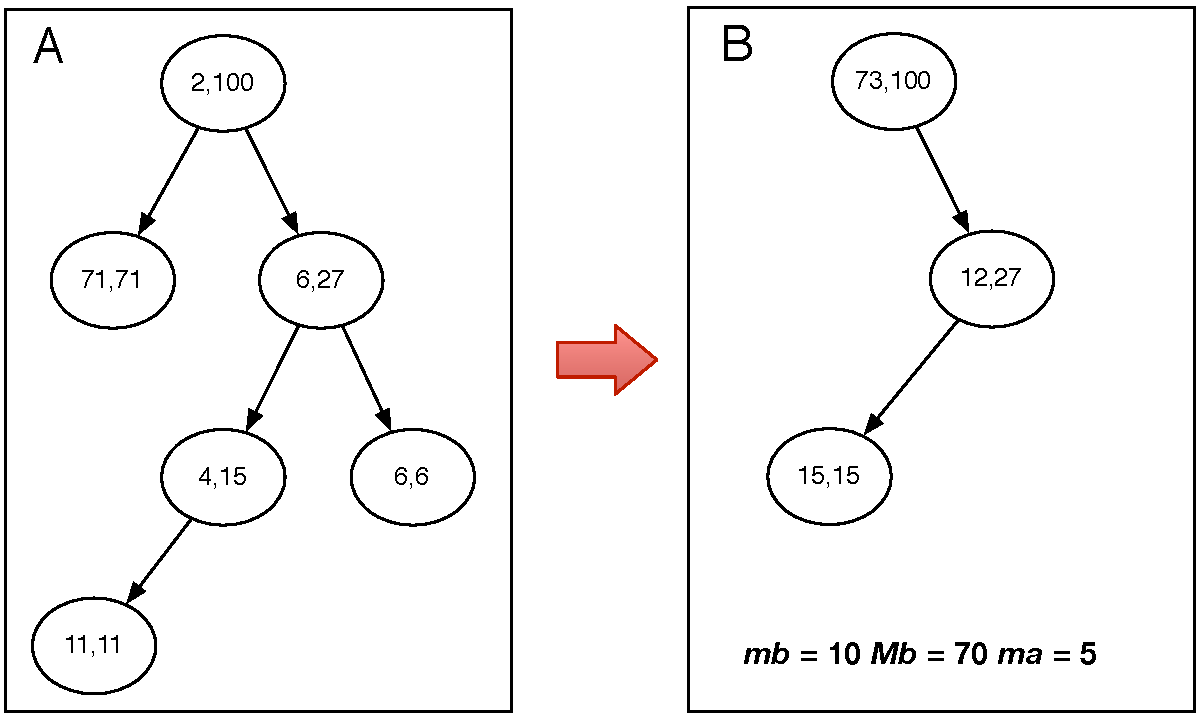
\includegraphics[width=1.0\textwidth]{images/cptree_pruning}
\caption[Demo of component tree pruning]{The demo of component tree pruning with $mb$, $Mb$, and $ma$ thresholding. Each node in the tree is labelled as its $\alpha$ size and $\beta$ size.}
\label{fig:cptree-pruning}
\end{figure}

\subsection{Application for image filtering} \label{sec:cptree-applic}
As mentioned in the sec.\ref{sec:thresh-cptree}, component tree is considered to be an advanced thresholding techniques, which is the collection of all possible thresholding components. A major use of the component tree is for image filtering \cite{najman2006building}. Fig.\ref{fig:cptree-flywing} shows the filtering result of a fly wing image. The intensity of wings increase gradually from bottom-left to top-right. It is impossible to segment the objects out with single threshold. With pruned component tree, we can get the filtering result by keeping only leaf nodes.

\begin{figure}[htbp]
\centering
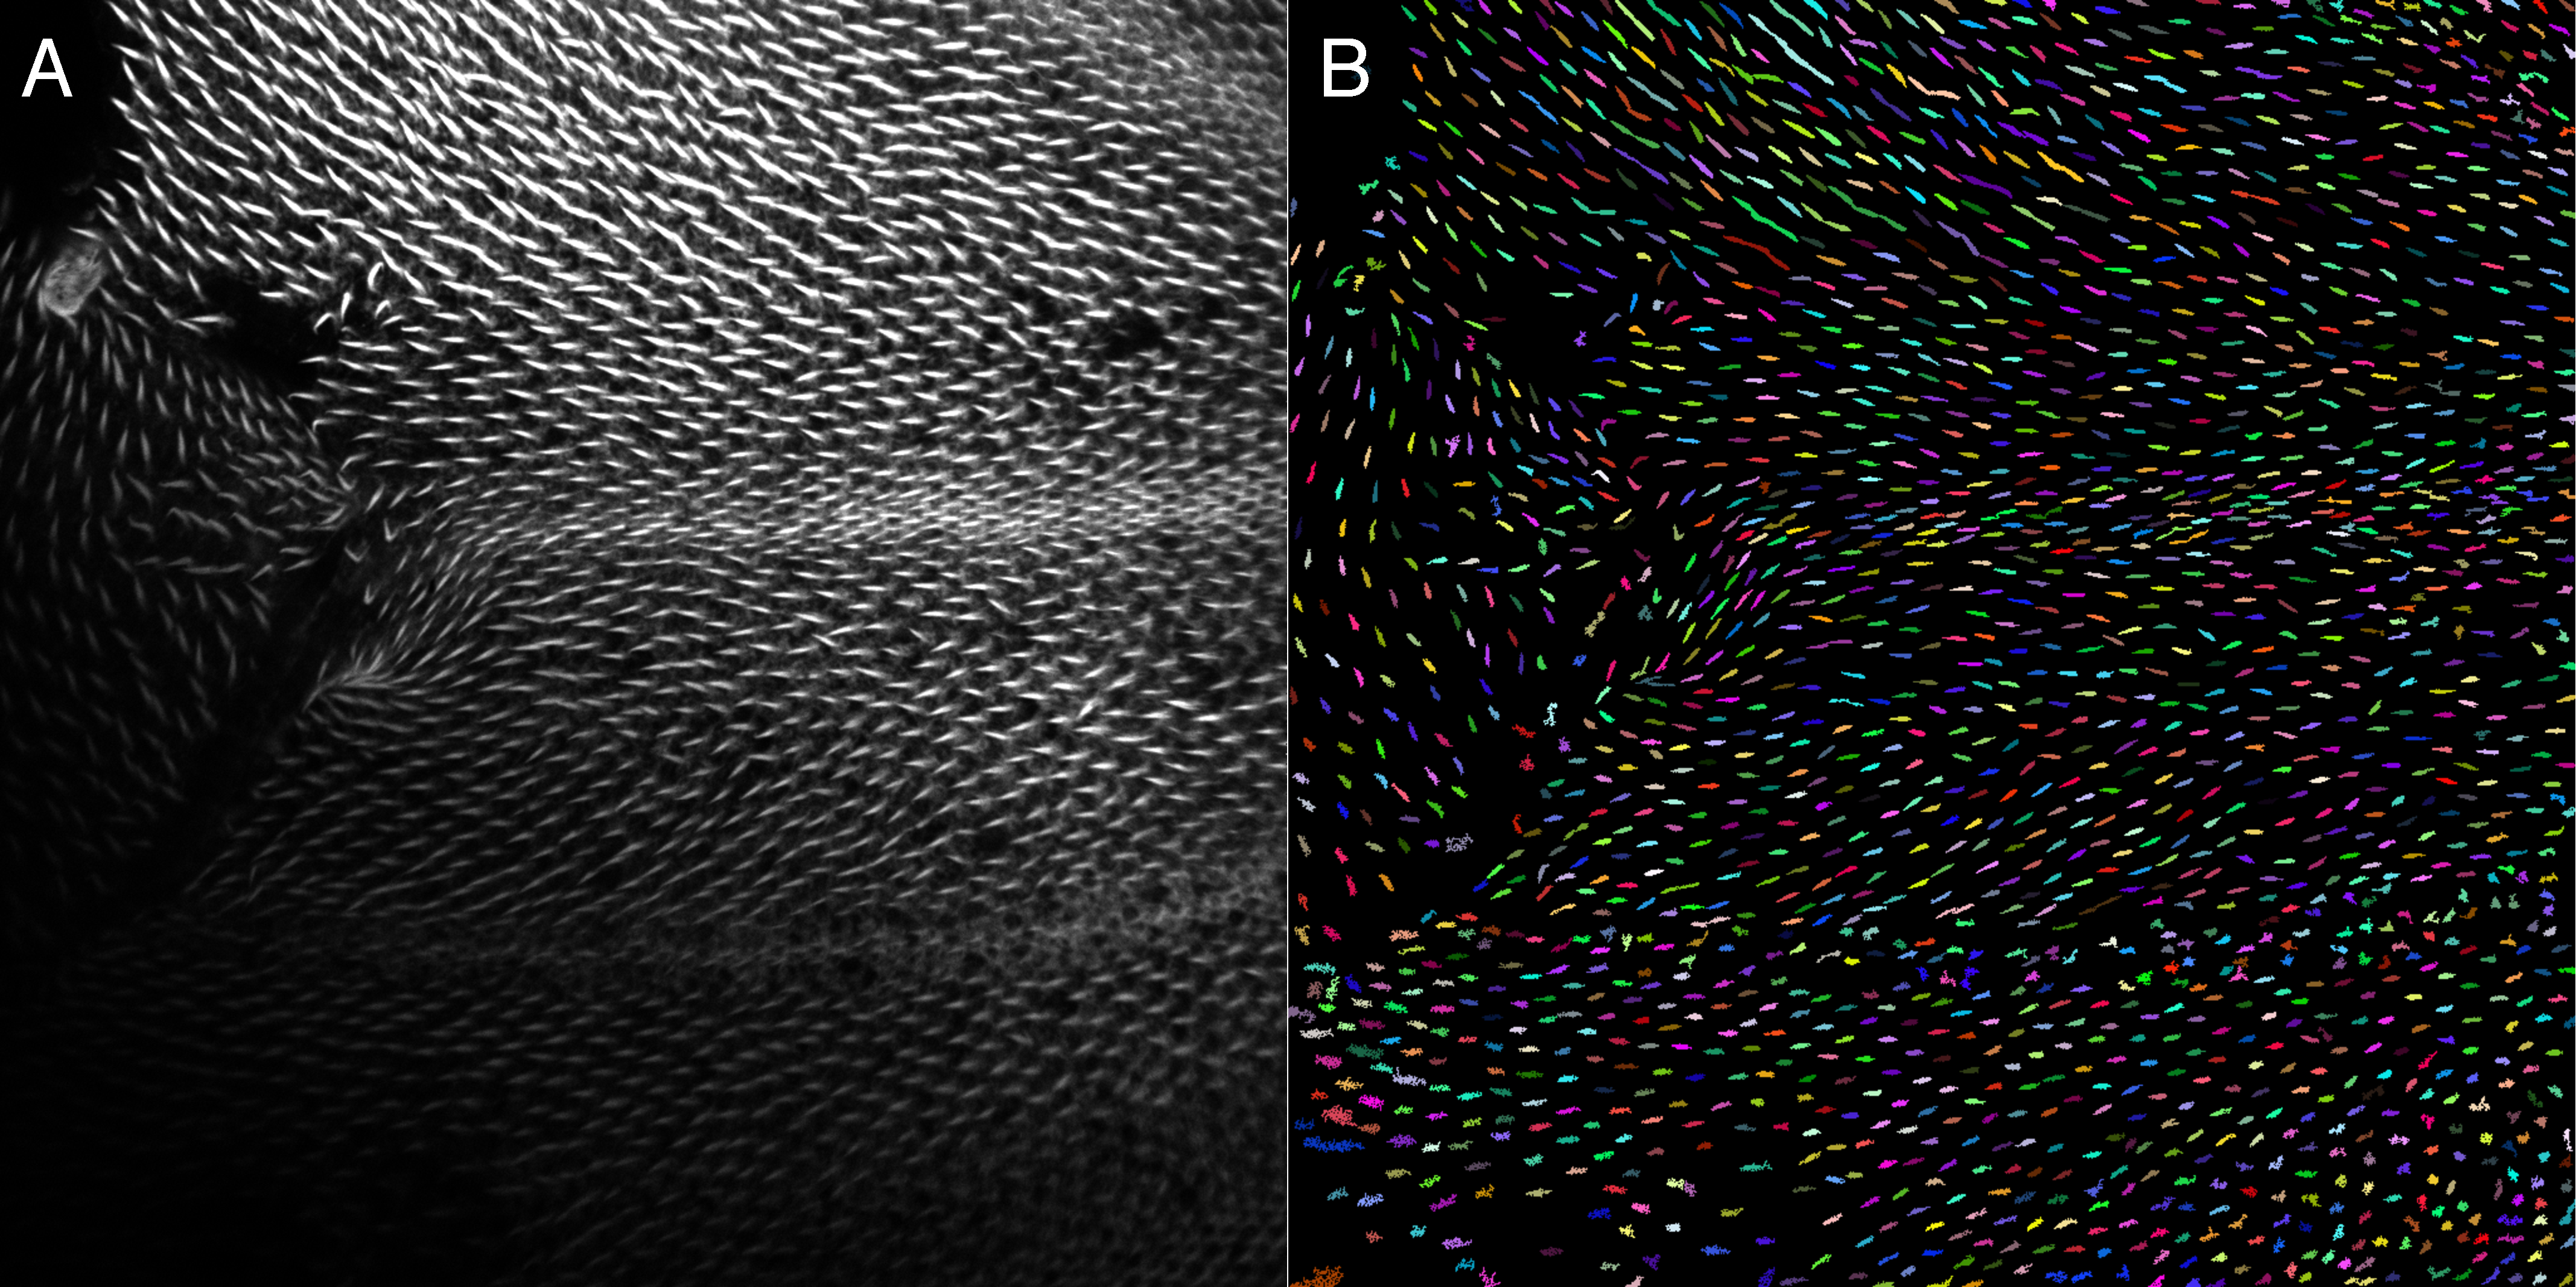
\includegraphics[width=1.0\textwidth]{images/cptree_flywing}
\caption[Filtering result of fly wing by keeping only the child nodes of the pruned component tree]{Filtering result of fly wing (1024x1024) by keeping only the child nodes of the pruned component tree. After pruning with parameter mb = 50, ma = 1, and Mb = 100000, the component tree contains 72209 nodes. And there are 2063 wing hairs left. A. the gray-scale wing fly image. B. the segmented result.}
\label{fig:cptree-flywing}
\end{figure}

\section{Weights between component trees} \label{sec:cptree-weight}
\subsection{Weighting function}
An important part of obtaining cosegmentation is to compute the nodes weights between two given component trees $S$ and $T$. A weighting function to be used for cosegmentation, as introduced in \cite{Xiao:2011, xiao2011dynamic}, is the Jaccard index (or Tanimoto score):
$$
w_{u,v} = \frac{|\beta(u) \cap \beta(v)|}{|\beta(u) \cup \beta(v)|}
$$
where $u$ and $v$ are nodes from $S$ and $T$ respectively, $\beta(u)$ and $\beta(v)$ are the beta area of the node $u$ and node $v$.

\subsection{Dynamic process for weight calculation}
Before computing tree assignments between two trees, the weight between each pair of nodes, one in each component tree, needs to be computed. In practice, calculating weights is a major bottleneck for computing cosegmentations. Here, we propose a linear time dynamic programming algorithm for calculating overlap weights by systematically utilizing the inclusion relationship of a node and its children in a component tree.

For each node $v$, $\beta(v)$ is the connected area in the image that is
associated with $v$, while $\alpha(v)$ is the connected area of $v$
\emph{excluding} the connect areas of the \emph{children of} $v$. The 
pixels in $\alpha(v)$ belong \emph{exclusively} to $v$ and not to any of its
children. Furthermore, let $v_i$ denote the $i$-th child of node $v$ and
$C(v)$ be the set of children of $v$. Then, we have
\begin{equation*} \label{eqn:beta-disjoint}
\beta(v_i)\cap\beta(v_j)=\emptyset\quad\mbox{for all $v_i\neq v_j\in C(v)$}
\end{equation*}
Hence, $\beta(v)$ can be decomposed as follows:
\begin{equation*} \label{eqn:beta-decompose}
\beta(v) = \alpha(v)\cup\bigcup_{v_i \in C(v)} \beta(v_i)   
\end{equation*}

That is to say, $\beta(v)$ can be \emph{partitioned} into $\alpha(v)$ and
$\beta(v_i)$, $v_i \in C(v)$.  This will be the guiding principle of our
dynamic programing algorithm for weight calculation.

Let $S=(V_S,E_S,\alpha,\beta)$ be the first component tree, and
$T=(V_T,E_T,\alpha,\beta)$ be the second component tree. Our task is to compute
the Jaccard index between each vertex $u$ in $S$ and vertex $v$ in $T$, defined
as
\begin{equation*}
w(u,v) = |\beta(u) \cap \beta(v)| ~/~ |\beta(u) \cup \beta(v)|
\end{equation*}
We can rewrite the above as
\begin{equation*}\label{eqn:jaccard-rephrase}
w(u,v) = \frac{|\beta(u) \cap \beta(v)|}{|\beta(u)| + |\beta(v)| - |\beta(u) \cap \beta(v)|}
\end{equation*}
Thus, the weight calculation between vertex $u$ in $S$ and vertex $v$ in $T$ can
be rephrased as calculating intersections between $\beta(u)$ and $\beta(v)$. As
a shortcut notation, we denote the cardinality of the intersection of $\beta(u)$
and $\beta(v)$ as
\begin{equation*}
  \label{eqn:betabeta}
  \beta\beta(u,v) = |\beta(u) \cap \beta(v)|  
\end{equation*}

Similarly, we define 
\begin{equation*} \label{eqn:alphabeta}
\alpha\beta(u,v) = |\alpha(u) \cap \beta(v)|  
\end{equation*}
\begin{equation*} \label{eqn:alphaalpha}
\alpha\alpha(u,v) = |\alpha(u)\cap\alpha(v)|
\end{equation*}

Decomposing $\beta(v)$ into $\alpha(v)$ and $\beta(v_i)$, we can split $\beta\beta(u,v)$ into

\begin{equation*} \label{eqn:betabeta-comp}
\beta\beta(u,v) = \alpha\beta(u,v) + \sum_{u_i \in C(u)}\beta\beta(u_i,v),
\end{equation*}
while $\alpha\beta(u,v)$ can be decomposed into
\begin{equation*} \label{eqn:alphabeta-comp}
\alpha\beta(u,v) = \alpha\alpha(u,v) + \sum_{v_i \in C(v)}\alpha\beta(u,v_i),
\end{equation*}

For our dynamic programming algorithm, the idea is to use three dynamic
programming tables $\alpha\alpha$, $\alpha\beta$, and $\beta\beta$. Based on the
dependency relationship between them, we compute them in the following
order:
\begin{equation*}
\alpha\alpha(u,v) \to \alpha\beta(u,v) \to \beta\beta(u,v)  
\end{equation*}

Let $P$ be the set of all pixels in an image, and $T(V,E,\alpha,\beta)$
be its component tree. Then, $\alpha(v)$ is a partition of $P$
\begin{equation} \label{eqn:alpha-decompose}
P = \bigcup_{v \in V}\alpha(v)
\end{equation}

This allows us to define a reverse mapping of $\alpha^{-1}: P \to V$ that
identifies for each pixel $p\in P$, the unique vertex $v$ that satisfying
$p\in\alpha(v)$.  This reverse mapping allows us to calculate all
$\alpha\alpha(u,v)$ in time $O(|P|)$. Fig.\ref{fig:cptree-aaweight} illustrates
the decomposition of $\alpha\alpha$ weight calculating.

\begin{figure}[htbp]
\centering
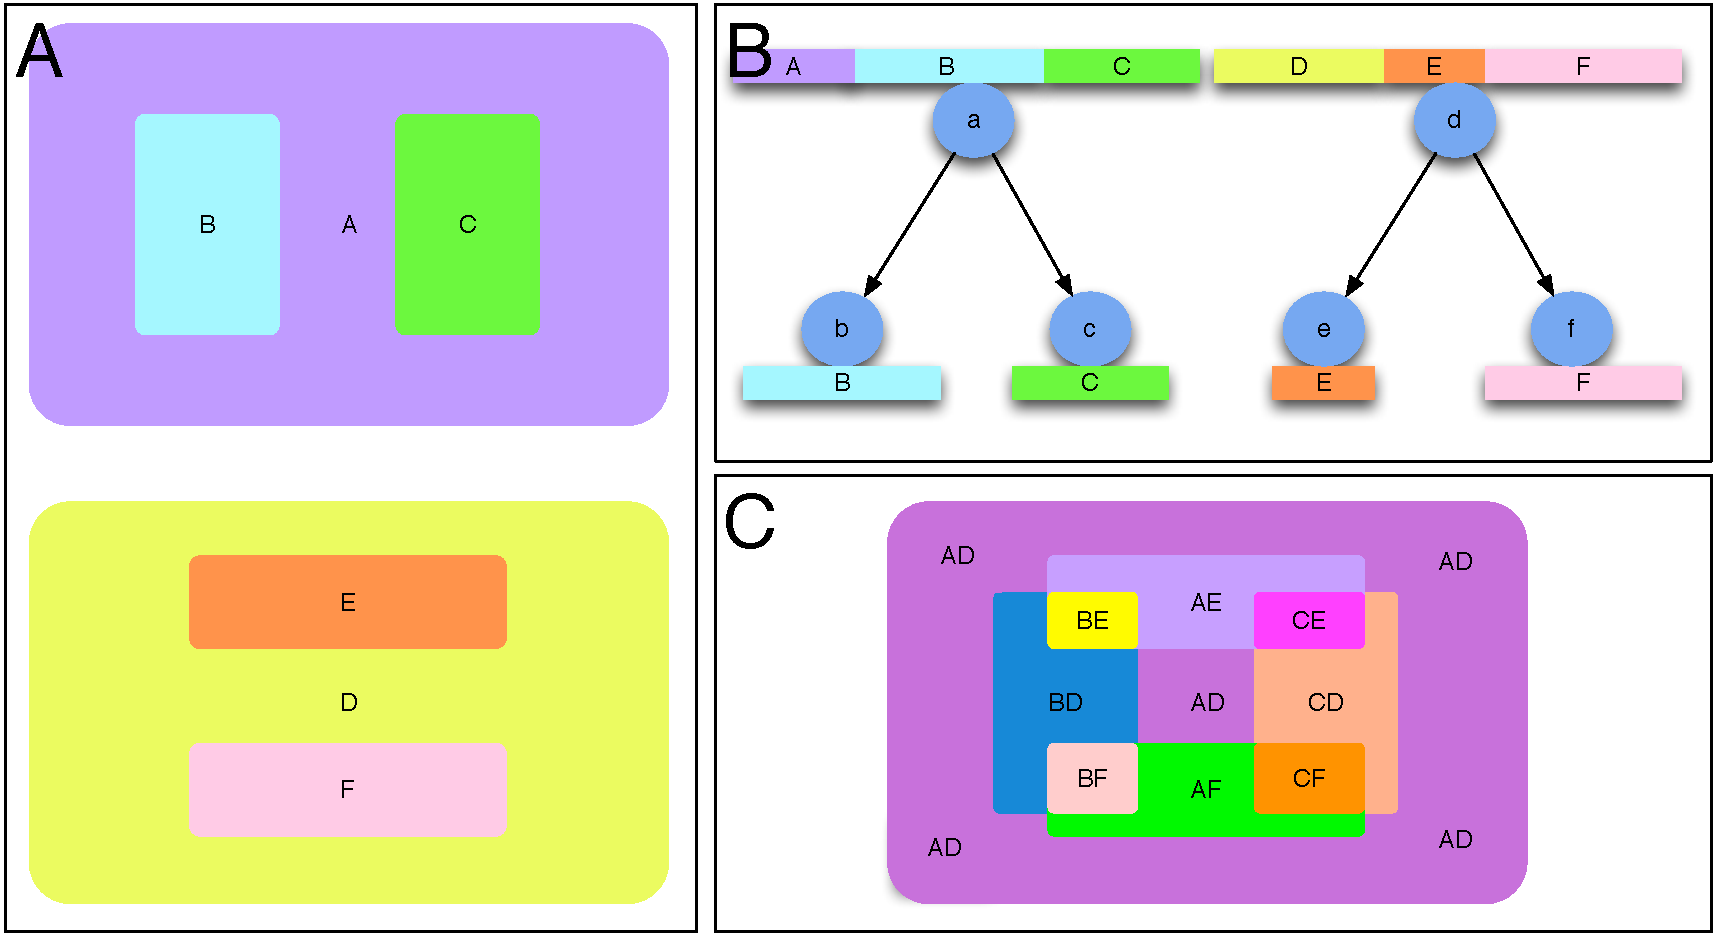
\includegraphics[width=1.0\textwidth]{images/cptree_aaweight}
\caption[The decomposition of $\alpha\alpha$ weights between two simple component
trees.]{The decomposition of $\alpha\alpha$ weights between two simple component
trees. A. The compents of two images; B. The component trees of the two images. 
The small case denotes the component node, whereas the large case denotes the $\alpha$
area; C. The overlapping $\alpha\alpha$ areas. Each image pixel is mapped to a 
component node in both component tree.}
\label{fig:cptree-aaweight}
\end{figure}

Based on the above recurrence relations, both $\beta\beta(u,v)$ and
$\alpha\beta(u,v)$ can be calculated in a dynamic programming fashion by
postorder traversal of the component trees (see Algorithm 1). This leads to a
time complexity of $O(|S| \cdot |T)$.  

\subsection{Quasi-linear running time}
\paragraph{Worst-case time complexity.} For the whole weight calculation
process, we first compute all $\alpha\alpha$ weights, then the
$\alpha\beta$ weights, and finally the $\beta\beta$ weights, yielding
a total running time of $O(|P| + |S|\cdot|T|)$.  

\def\avg{\mathrm{avg}}

From Eqn.~\eqref{eqn:alpha-decompose}, we get
\begin{equation*}
|V| = \frac{|P|}{\avg_{v\in V}(|\alpha(v)|)} 
\end{equation*}

We always have $|V|\le|P|$, since $\avg_{v\in V}(|\alpha(v)|) \ge 1$.
For large images ($|P| \sim 10^6$) such as the ones considered in Section
\ref{sect:results}, the full component tree contains about $10^5$ vertices.  
However, after pruning, the tree size decreases dramatically, to typically much
less than $500$, as observed in \cite{Xiao:2011}.  
Usually, for large images, we have $\avg_{v\in V}(|\alpha(v)|) > |V|$, so $|V|^2
\ll |P|$. Under these circumstances, the total running time, dominated by the
number of pixels, is quasi-linear w.r.t $|P|$.

\begin{algorithm}[H]
\SetAlgoLined
\KwData{Component tree $S$ and $T$ with $\alpha$ size and $\beta$ size}
\KwResult{All pair of weights between nodes and $S$ and nodes in $T$}
Compute post-order enumerations of the nodes in $S$ and $T$ as $u_1,\ldots,u_n$ and $v_1, \ldots, v_m$, respectively\;
\emph{\{$\alpha\alpha$ weights calculation\}}\;
Initialize all $\alpha\alpha(u,v)$ to 0\;
\ForEach{pixel $p \in P$ do}{
  $u := \alpha_1^{-1}(p)$\;
  $v := \alpha_2^{-1}(p)$\;
  increase $\alpha\alpha(u,v)$ by one\;
}
\emph{\{$\alpha\beta$ weights calculation\}}\;
\For {$i$ from 1 to $n$ }{
	\For {$j$ from 1 to $m$}{
		Initialize $\alpha\beta(u_i,v_j)$ to $\alpha(u_i,v_j)$\;
		\ForEach {child $c \in C(v_j)$}{
		  $\alpha\beta(u_i,v_j) := \alpha\beta(u_i,v_j) + \alpha\beta(u_i, c)$\;
		}
	}
}
\emph{$\beta\beta$ weights and Jaccard index calculation}\;
\For {$i$ from 1 to $n$}{
  \For {$j$ from 1 to $m$}{
  	Initialize $\beta\beta(u_i,v_j)$ to $\alpha\beta(u_i,v_j)$\;
	\ForEach{child $c \in C(u_i)$}{
	  $\beta\beta(u_i,v_j) := \beta\beta(u_i,v_j) + \beta\beta(c,v_j)$\;
	}
  }
}
\caption{Computing all overlap weights between component trees $S$ and $T$}
\label{alg:cptree-weights}
\end{algorithm}
